\chapter{Motivation}\label{motivation}
Der stetig steigende Fachkräftemangel trifft auch das Baugwerbe. 
Laut einer Umfrage des Hauptverbandes der Deutschen Bauindustrie e.V. stufen über 75 Prozent aller befragten Unternehmen sowohl den vorherrschenden Fachkräftemangel, als auch die steigenden Energie- und Rohstoffpreise als Risiko für das eigene wirtschaftliche Wachstum ein \cite{Bauindustrie:online}.
Abbildung~\ref{fig:Fachkraeftemangel} illustriert die Entwicklung dieser Sorge über einen Zeitraum von etwas mehr als zwanzig Jahren.
Damit ist es wenig überraschend, dass eine Bewegung weg von menschlichen Arbeitskräften hin zur Automatisierung existiert.
Neben dem Fachkräftemangel stellt aber auch die geringe Effizienz von Bauvorhaben ein Problem dar, welche sich über den gesamten Planungs- und Bauprozess erstreckt. 
Diese Ineffizienz entsteht aufgrund der Vielzahl der an Bauprojekten beteiligten Experten und Unternehmen.
Dies ist ein bekanntes Problem und wird als \textit{Fragmentierungsproblem der Bauindustrie} bezeichnet~\cite{ConstructionFragmentation}.
\begin{figure}[h]
    \centering
    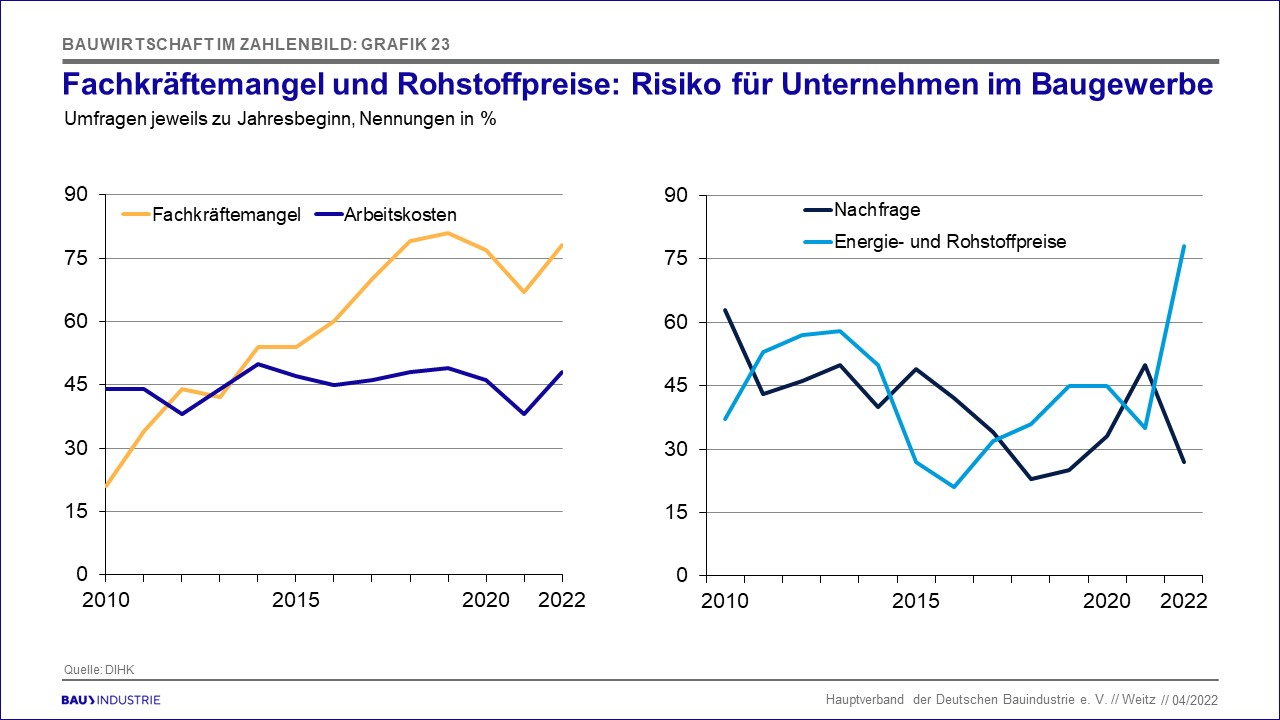
\includegraphics[width=0.7\columnwidth]{fig/Grafik_23.jpg}
    \caption{Während wirtschaftliches Risiko durch eine potentiell sinkende Nachfrage nach Bauafträgen und eventuell steigender Arbeitskosten unverändert blieben oder sogar als weniger relevant bewertet wurden, ist ein deutlicher Anstieg aufgrund des vorherrschenden Fachkräftemangels und der Energie- und Rohstoffpreise zu erkennen.}
    \label{fig:Fachkraeftemangel}
\end{figure}
Um dem entgegenzuwirken, etablieren sich bereits seit einigen Jahren Standards, um Bauprojekte digital zu begleiten.
Mit diesen soll gleichzeitig die Effizienz gesteigert, die Kommunikation zwischen den einzelnen Expertenteams vereinfacht, der Arbeitsplatz \glqq{}Baustelle\grqq{} sicherer gestaltet und ein resourcensparender Bau ermöglicht werden~\cite{BIMforHe12:online}\cite{Top10Ben31:online}.
Zusätzlich steigen mit der Zunahme an digitalen Informationen zu Bauprojekten, auch die Möglichkeiten diese ausführlicher zu analysieren, zu optimieren und an neue Technologien zu knüpfen.
Erst dadurch wurde das seit einigen Jahren erforschte Gebiet der \textit{Additiven Fertigung} von Gebäuden realisierbar.
Einige erfolgreiche Beispiele dafür sind in~\cite{AdditiveManufactoringDelgado},~\cite{AdditiveManufacturingUsingMobileRobots} und~\cite{Tankova2020} aufgezeigt und wurden etwa mit Beton druckenden Roboterarmen, mobilen Robotern oder aufgehängten Druckköpfen durchgeführt.
Dabei werden teils herkömmliche, teils speziell für die druckenden Roboter entwickelte Materialien verwendet~\cite{Tankova2020}.
Obwohl es mittlerweile viele Projekte zur Additiven Fertigung von Gebäuden gibt, haben diese oft den Nachteil der Nicht-Parallelisierbarkeit der druckenden Roboter und die daraus resultierende, vergleichsweise lange Bauzeit.
Auch die durch die Höhe der temporären Stützstrukturen (wie Kräne, Gerüste oder Aufhängungen) eingeschränkte Bauhöhe limitiert die Vielfalt der mit additiver Fertigung realisierbaren Projekte.
Diesen Einschränkungen soll nun mithilfe eines Schwarmes bodengebundener automoner Roboter, die gleichzeitig an dem Bauprojekt arbeiten können, entgegengewirkt werden.
Dabei sollen sich die Roboter auf den Mauern des Gebäudes selbst bewegen können, während sie diese errichten.
Im Gegensatz zur additiven Fertigung sollen die Roboter das Material nicht etwa drucken, sondern herkömmliche Bausteine verweden können.
In dieser Arbeit liegt der Schwerpunkt allerdings nicht auf der Entwicklung dieser Roboter, sondern auf dem Erarbeiten eines Vorgehens zur Berechnung von für Roboterschwärme geeigneten Bauplänen, ausgehend von 3D Modellen der Gebäude.
Dies stellt die Grundlage für nachfolgende Automatisierungsprojekte im Bereich der Bauindustrie dar.
Das Anfertigen der Modelle innerhalb eines 3D Editors ermöglicht nicht nur das Definieren geometrischer und physikalischer Eigenschaften eines Gebäudes in digitaler Form, sondern verschlankt zudem die Kommunikation zwischen Endnutzer und Architekturbüro oder ersetzt letzteres komplett.
Gleichzeitig macht diese Arbeit damit einen Schritt in Richtung des relativ neuen Trends der sogennanten Massenpersonalisierung, welcher als Nachfolgetrend zur Massenproduktion und als \glqq{}heilger Gral\grqq{} der Fertigung angesehen wird~\cite{MassCustomHolyGrail}.
Dieser Trend ist auch für die Bauindustrie interessant, denn auch hier schafft die Möglichkeit sämtliche Kundenwünsche an ein Produkt (oder in diesem Fall ein Gebäude) umzusetzen, ohne dafür spezielles Werkzeug herstellen oder Verfahren entwickeln zu müssen, neue Gewinnmöglichkeiten~\cite{Jensen2018}~\cite{Jensen2015}.
Dennoch existiert noch vergleichsweise wenig Forschung die teilweise schon etablierte Konzepte der Massenpersonalisierung aus der Fertigungsindustrie ebenfalls in der Bauindustrie zu erproben~\cite{Larsen2019}.
Darum soll in dieser Arbeit untersucht werden, in welcher Weise sich bereits vorhandene digitale Standards und Austauschformate dafür eigenen, individuelle Baupläne aus den 3D Plänen von Gebäuden zu generieren.
Die Baupläne können dabei aufgrund der Anbindung an einen frei verfügbaren 3D Editor nicht nur von Experten, sondern ebenfalls von Laien stammen.
So kann ein Endnutzer persönliche Wünsche selbst in das Modell integrieren.
Zudem wird nach einer Möglichkeit gesucht, die resultierenden Baupläne durch adaptive Regelsets an die jeweilige Situation anpassen zu können, denn unterschiedliche Bauprojekte besitzen oft unterschiedliche Eigenheiten und Prioritäten.
Diese Konzepte werden daraufhin anhand nachfolgender Fallstudien getestet.